\documentclass[11pt]{article}

\parindent=10pt
\parskip=6pt
\usepackage[paper=a4paper, left=2cm, right=2cm, bottom=2.5cm,top=2.5cm]{geometry}

% Paquetes de nacionalización. No olvidar para poder poner tildes!
\usepackage[spanish]{babel}
\usepackage[utf8]{inputenc}
\usepackage{listingsutf8}

% Paquetes para pseudo
\usepackage{listings} % este es para codigo posta
\usepackage[usenames,dvipsnames,svgnames,table]{xcolor}

% Paquete para imagenes
\usepackage{float}

% Caratula (Recordar logo_uba.jpg y logo_dc.jpg)
\usepackage{caratula}

% Bibliografia
\usepackage{biblatex}
\addbibresource{biblio.bib}

% Color de links
\usepackage{hyperref}
\hypersetup{
    colorlinks,
    citecolor=black,
    filecolor=black,
    linkcolor=black,
    urlcolor=black
}

\begin{document}


\materia{Seguridad de la Información}
\submateria{Primer Cuatrimestre 2016}
\titulo{Investigación en seguridad en procesos\\ electorales}
\subtitulo{TP final}
\integrante{Brian Litwak}{241/12}{brian.litwak@gmail.com}
\integrante{Gino Scarpino}{}{gino.scarpino@gmail.com}
\integrante{Silvio Vileriño}{106/12}{svilerino@gmail.com}
\integrante{Valeria Tiffenberg}{193/10}{valetiff@gmail.com}


\maketitle
\pagebreak

\tableofcontents

\pagebreak

\section{Introducción}

En este trabajo se quiere presentar un panorama de la evolución de los sistemas electorales informáticos, tomando los ejemplos de varios países y haciendo hincapié en sus aciertos y errores de seguridad.

Dentro de los sistemas electrónicos de votación, reconocemos dos categorías: el voto electrónico presencial, ejemplificado por el que se dio en las últimas elecciones en la Ciudad de Buenos Aires, y el voto por internet, como lo ha tenido Suiza desde fines de la década del 90\cite{gerlach}.

La historia de los sistemas elctrónicos de votación empieza mucho antes que en la Argentina. Sin ir más lejos, Brasil tiene su sistema en funcionamiento desde el año 96\cite{corteBrasil}. Otros países con sistemas activos son India, Perú, Colombia, Estados Unidos, Francia y Japón, y ha habido algunos países donde se usó por varios años y decidió discontinuarse, y otros donde se han hecho pilotos que finalizaron en la decisión de no aplicar el sistema\cite{ndi}.

En este informe todos estos casos resultan de interés, con foco particular en el uso argentino. En el desarrollo del informe se irán mencionando otras experiencias para completar el panorama global relacionado con el voto electrónico.

\section{Temas a desarrollar}

Intentaremos hacer hincapié separadamente en los problemas posibles dentro de la seguridad informática: confidencialidad, integridad y disponibilidad, para tratar de abarcar toda la superficie de vulnerabilidades. Para ordenar el trabajo, se van a usar los grupos sugeridos en el enunciado:

\begin{itemize}
\item Estándares de almacenamiento de votos (Puede afectar disponibilidad e integridad)
\item Seguridad física de las maquinas de votación (integridad)
\item Transmisión de votos para su posterior escrutinio (afecta confidencialidad e integridad)
\item Privacidad del voto (afecta confidencialidad e integridad)
\item Auditabilidad del sistema  (afecta disponibilidad y confidencialidad)
\item Comprobantes
\end{itemize}

Los tres ángulos de la seguridad informática son fundamentales a la confianza en las elecciones electrónicas, y la confianza es, discutiblemente, el pilar sobre el que las elecciones democtráticas suceden. Así como en muchos países no es obligatorio ir a votar, son aquellos que sí confían en que el resultado generará alguna diferencia y tiene importancia, quiénes se acercan a las urnas, digitales o no.

La confidencialidad está establecida por ley en aquellos países que hemos investigado: el voto es secreto para proteger a la persona de ataques o influencias, y que vote a quién realmente desea votar. Las interfaces electrónicas de votación deben garantizar que al momento de votar, nadie más que el votante sabe el voto, y al mismo tiempo, que el almacenamiento de los votos y de la lista de votantes no se pueden unir, a posteriori, para asociar un voto a una persona.

La integridad es, en este contexto, lo más importante para la confianza. Es necesario que el voto que la persona emitió sea contado como tal, ni por otro votante, ni mútiples veces, ni ignorado. El dato como se emitió, debe llegar a destino.

Por último, la disponibilidad tiene varios factores: por un lado es importante que hardware y software de votación estén en funcionamiento correcto al momento de realizarse las elecciones, para todos los votantes; y por otro, es necesario que los votos puedan ser contados para el recuento original, pero incluso que estén disponibles para nuevos recuentos si la justicia lo requiriera, por ejemplo.

\pagebreak
\section{Estándares de almacenamiento de votos}
El almacenamiento de votos es importante a corto y largo plazo. Es necesario poder obtener un resultado correcto al momento de finalizar la elección, pero también deben estar disponibles los datos si se quisiera hacer un recuento en el futuro.
Por lo visto, no hay una única forma de almacenar los votos durante el sufragio y se utilizan diversas formas para ello. Desde distintos medios de almacenamiento como tarjetas RIFT hasta la propia memoria de la máquina de votación, donde no necesariamente es excluyente alguna de las dos.
Mencionaremos distintas técnicas que se utilizaron en distintos países, y los agujeros de seguridad que se encontraron en tales.

\subsection{Estados Unidos}
En este país encontramos un caso que nos llama la atención ya que se utiliza criptografía en el voto electrónico, pero no es utilizada correctamente. Como dice el paper
\footnote{\url{http://www.engr.uconn.edu/~sad06005/pubs/Conference/sac12.pdf}}
que leímos sobre esta votación, la mera utilización de herramientas criptográficas puede conducir a una falsa sensación de seguridad. Con el fin de ser eficaz, la criptografía debe ser utilizada en conjunción con un buen diseño que proporcione una protección completa en la integridad de la información crítica.

En el paper mencionado, cuenta que para emitir votos de forma electrónica se utilizó la terminal de votación AccuVote TSX, utilizada por más de 12 millones de votantes en más de 350 jurisdicciones en los Estados Unidos. Los votos son almacenados en una tarjeta PCMCIA.

Esta terminal tiene vulnerabilidades que permiten un ataque que intercambia los votos de dos candidatos y otro que borra el nombre de un candidato. Ambos ataques son capaces de eludir las comprobaciones de integridad de cifrado implementados en la terminal. Los ataques se pueden iniciar en cuestión de minutos y sólo requieren una computadora con la capacidad para montar una tarjeta PCMCIA. No es necesario que el atacante tenga información de la elección que va a modificar, sólo es necesario que tenga acceso a la maquina de votación para abrir el compartimiento donde se almacena la tarjeta PCMCIA.

Las vulnerabilidades encontradas en el paper fueron:
\begin{itemize}
	\item Aunque el nombre de cada candidato está acompañado por 128 bits de integridad, la terminal no los usa de forma efectiva. Cuando falla el chequeo de integridad en un candidato, no se cuenta el voto para este candidato. Aunque el elector verifique en la boleta VVPAT que figura el candidato de forma correcta, su voto no será tenido en cuenta para el recuento de votos ya que el recuento electrónico lo realiza con lo almacenado en la tarjeta PCMCIA y al fallar la integridad del candidato, no lo cuenta. Tampoco existe una verificación de la integridad de que no se cambió los nombres de candidatos en los recuentos de los votos
	\item No hay una firma criptográfica de la tarjeta PCMCIA. Por ende, se puede agregar más contenido a la urna de votación
	\item La existencia de puertas traseras como en versiones anteriores de la terminal y un mecanismo de actualización de archivos débil ya que tan solo se utiliza el nombre del archivo a actualizar para identificar una actualización de software válida
	\item Las máquinas de votación tienen la misma llave física para obtener la tarjeta PCMCIA, al menos en las que fueron revisadas
\end{itemize}

Otra falla relacionada al almacenamiento, que existió en Estados Unidos durante una elección
\footnote{\url{http://usatoday30.usatoday.com/news/politicselections/vote2004/2004-11-04-votes-lost_x.htm}}
 utilizando el voto electrónico, fue que más de 4.500 votos se perdieron en un condado de Carolina del Norte, porque las autoridades creían que una máquina de votación electrónica podía contener más datos que los que efectivamente almacenaba.

\subsection{India}
Este país nos resultó interesante ya que es el país democrático que utiliza el voto electrónico con mayor cantidad de población. En elecciones nacionales recientes, fueron contados más votos que juntando la población de Estados Unidos y Canadá, y la mayoría de los electores votaron utilizando el voto electrónico.
El componente electrónico de votación en India, llamado EVM, está compuesto por dos partes: la unidad de votación (izquierda) y la unidad de control (derecha) que están enlazadas por un cable de 5 metros. Las unidades de votación están realizadas para soportar hasta 16 candidatos. En caso de ser más candidatos, se agrega otra unidad de votación y es posible agregar hasta 4 unidades de votación, dando una capacidad máxima de 64 posibles candidatos. En la unidad de votación, se agrega una hoja indicando que botón representa a cada candidato con el símbolo de su partido político. Para votar, el elector tiene que ser identificado por el presidente de mesa que luego le realiza una marca en el dedo con tinta indeleble para evitar que vuelva a votar y presiona un botón en la unidad de control, permitiendo al elector votar en la unidad de votación. Al realizar esto, se prende una luz en la unidad de votación indicando que el votante está listo para sufragar.

\begin{figure}[h]
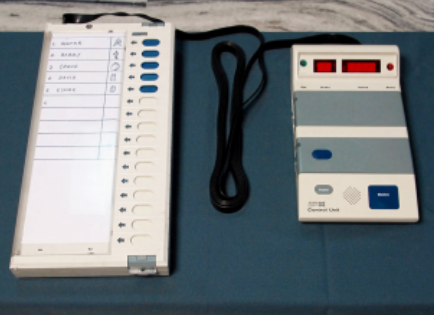
\includegraphics{Imagenes/almacenamiento1}
\caption{Máquina de votación electrónica utilizada en India}
\end{figure}

Las vulnerabilidad encontrada en el paper leído es
\footnote{\url{https://jhalderm.com/pub/papers/evm-ccs10.pdf}}
que se puede reemplazar fácilmente algún componente del equipo sea CPU, placas o agregar hardware. Los diseñadores de las EVM podrían haber hecho los ataques más difíciles agregando un mecanismo criptográfico para identificar a los distintos componentes de hardware originales, como un mecanismo de challenge response basado en un secreto contenido en el firmware original.

Uno de los posibles ataques mencionados en el paper es Dishonest Display. Se desarrolló una placa de visualización que puede reemplazar a la placa real en la unidad de control. Normalmente, cuando los votos son contados, la cantidad de votos recibidos por cada candidato figura en el tablero real. Con el ataque, el tablero agrega un microcontrolador que intercepta los votos totales y realiza la sustitución fraudulenta de resultados emitiéndose en el tablero de visualización. Notar que en este ataque hay que realizar un intercambio de un componente de hardware.

\begin{figure}[h]
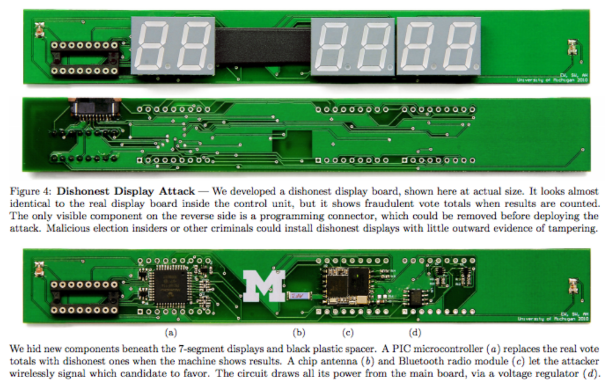
\includegraphics[width=0.8\textwidth]{Imagenes/almacenamiento2}
\caption{Hardware utilizado}
\end{figure}

%Además, el paper menciona otro ataque más pero optamos comentarlo en la sección de privacidad ya que tiene más relación con la pérdida del anonimato.
Un detalle no menor, es que el recuento de votos de la elección en India se realiza semanas después del sufragio. Por ende, el atacante tiene tiempo para poder realizar el cambio o agregar hardware que le permite realizar el ataque mientras están almacenadas.

\subsection{Holanda}
% Este país
% \footnote{\url{https://www.ndi.org/e-voting-guide/netherlands-CS/opposition-to-e-voting}}
% \footnote{\url{http://wijvertrouwenstemcomputersniet.nl/English}}
%  nos llamó la atención porque debido la fuerza mediática que tuvo en la sociedad la difusión de un video
% \footnote{\url{http://www.veoh.com/watch/v505707dgewqMsB}}
%  sobre las máquinas de votación NEDAP podían ser manipuladas, se logró volver a votar en papel y lápiz, como se votaba anteriormente en este país.
% Sucedió algo similar al caso de India: se necesitaban 5 minutos para poder manipular una de estas máquinas NEDAP cambiando dos chips, y como estas estaban guardadas sin una seguridad correspondiente al tema en cuestión, cualquier persona podia modificarlas.

\subsection{Argentina e Israel}
Otra forma de almacenar los votos, es la implementada en las elecciones del 2015 en Argentina y en las elecciones previas al 2010 en Israel, donde los votos se grababan en un chip RFID que se encontraba en la boleta (En el caso de Argentina sería la BUE) y se deposita la boleta en una urna física. Luego, en el escrutinio de votos, se utiliza una maquina para leer la información de la boleta y poder contabilizar el voto. En la sección de privacidad, seguiremos mencionando estos países ya que los comentarios acerca de los posibles ataques tienen más que ver con la pérdida del anonimato que con el formato de almacenamiento en si.


\pagebreak
\section{Seguridad física de las maquinas de votación}
Los accesos a la máquina proveen varias formas posibles de ataques: cuánto menos expongan entradas para posibles atacantes, más seguras serán. Por otro lado, se debe tener en cuenta la custodia de las máquinas: quién tiene acceso y cuándo, y si es posterior al último chequeo oficial. Así mismo, se tiene que contemplar y facilitar el acceso a todos los votantes.

\subsection{Acceso a información del hardware}

Para empezar es imprescindible contar con la información completa del sistema a utilizar: software, hardware, flujos, participantes, entre muchas otras cosas. Es necesario para poder auditar previo al hecho electoral, durante y posteriormente al mismo. La importancia de tener la información de cada componente interviniente del sistema, es poder investigar la presencia de vulnerabilidades conocidas o detectar alguna vulnerabilidad en la interacción entre componentes. Un claro ejemplo donde podemos contrastar es el caso de la empresa MSA (Magic Software Argentina), responsable de la votaciones realizadas en Salta y en la Ciudad de Buenos Aires. En su sitio, solo hay información superficial del sistema de votación, en cuanto a las máquinas, nada más que fotos e infografías. Por otra parte, una empresa internacional Smartmatic, dispone en cada producto un documento técnico con información específica de las máquinas\cite{smartmatic}, lo cual da mayor confianza. Esta última, fue la empresa responsable de las elecciones de La Falda y Marcos Juárez en Córdoba. La empresa afirma que obtuvieron en tiempo récord el escrutinio definitivo, y que fue de 45 minutos apróximadamente\cite{smartmatic:cordoba}.

En el caso de la Ciudad de Buenos Aires, esto se establece en el artículo 24, inciso b, de la Ley 4894. En las etapas previas al acto electoral, es decir, al uso del sistema Vot.ar, se realizaron varias auditorías.
En la auditoría de Claudio Riguetti, por la FCEN, se aclara lo siguiente: “Se destaca la falta de un Manual de Operaciones, que debería incluir todos los aspectos de configuración, instalación, despliegue, mantenimiento, repliegue y obtención y publicación de resultados”\cite{righetti}.

\subsection{Sistemas de control físico y contingencia}

La seguridad física no solo es restringir acceso a los componentes de la máquina, sino que se refiere también a los procedimientos y acciones para que no se violen los sistemas. Si se corrompe una máquina, destruye o algo similar, debería ser fácilmente recuperable o reemplazable. Se deben tener en cuenta mecanismos de contingencia previos y durante la votación. Algunas de las situaciones que se deberían tener en cuenta son incendios en las instalaciones, fallas con la corriente eléctrica, robo del equipamiento, fallas de fábrica o hardware, errores humanos como conteo doble de boletas, atentados, entre otros.

Es importante aprender de errores pasados, por lo que realizar estudios sobre elecciones previas puede aportar mejoras considerables. Para eso es necesario un registro minucioso de cada incidente, registrando casos con la mayor información posible. Un claro ejemplo, es la posibilidad de acceder físicamente a componentes de la máquina, por ejemplo en el caso de la Ciudad de Buenos Aires, la unidad de DVD está accesible, pero sobre todo, un puerto USB que podría permitir cargar algún tipo de script, como BadUSB\cite{votar}.

La EAC\footnote{Election Assistance Commission}, recomienda que ningún ente sea el propio validador de la seguridad de sus máquinas. Se debería de usar el principio de la responsabilidad compartida, es decir, que un agente externo examine y verifique.

Además, que hay que llevar un control estricto del personal, de los componentes que puede acceder y de los permisos sobre los mismos. Indudablemente, un control periódico de las máquinas es necesario, pero también de los lugares donde se lleva a cabo la votación. Al tener toda esa información, ayuda a tener un mejor control ante cualquier eventualidad. Un claro ejemplo, sería que en caso de incendio, como trasladar el equipo, resguardar la información, y cómo reanudar el acto electoral, una vez atacado correctamente el incidente.

Otra recomendación, es en el momento de diseñar el tema del almacenamiento, pensar a largo plazo. Considerar el espacio físico y los medios donde se podría alojar toda la información, políticas de seguridad sobre los mismos. Es necesario para las auditorías posteriores a la votación.

El estudio realizado por VITA acerca de un sistema de votación utilizado en Virginia, USA\cite{vita} registra vulnerabilidades físicas similares a las mencionadas anteriormente acerca de BUE.
La terminal de votación de este sistema, tiene una tapa protectora, que es fácilmente removible. Luego de remover esta carcasa, quedan expuestos puertos usb funcionales. Un ataque realizado por VITA consistió en hacer iniciar un sistema operativo desde una unidad USB y copiar las imágenes de los discos de la terminal.

\subsection{Ejemplo de ``tampering'' de componentes internos}

El componente electrónico de votación en India, llamado EVM, está compuesto por dos partes: la unidad de votación (izquierda \ref{fig:partsIndia}) y la unidad de control (derecha\ref{fig:partsIndia}) que están enlazadas por un cable de 5 metros. Las unidades de votación están realizadas para soportar hasta 16 candidatos. En caso de ser más candidatos, se agrega otra unidad de votación y es posible agregar hasta 4 unidades de votación, dando una capacidad máxima de 64 posibles candidatos. En la unidad de votación, se agrega una hoja indicando que botón representa a cada candidato con el símbolo de su partido político. Para votar, el elector tiene que ser identificado por el presidente de mesa que luego le realiza una marca en el dedo con tinta indeleble para evitar que vuelva a votar y presiona un botón en la unidad de control, permitiendo al elector votar en la unidad de votación. Al realizar esto, se prende una luz en la unidad de votación indicando que el votante está listo para sufragar.

\begin{figure}[H]
  \centering
  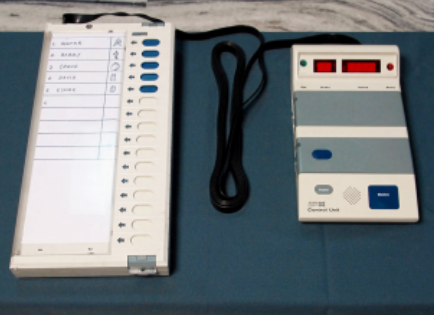
\includegraphics[scale=0.7]{Imagenes/almacenamiento1}
  \caption{Máquina de votación electrónica utilizada en India}
  \label{fig:partsIndia}
\end{figure}

Las vulnerabilidad encontrada en el paper leído es que se puede reemplazar fácilmente algún componente del equipo sea CPU, placas o agregar hardware\cite{india}. Los diseñadores de las EVM podrían haber hecho los ataques más difíciles agregando un mecanismo criptográfico para identificar a los distintos componentes de hardware originales, como un mecanismo de challenge response basado en un secreto contenido en el firmware original.

Uno de los posibles ataques mencionados en el paper es Dishonest Display. Se desarrolló una placa de visualización que puede reemplazar a la placa real en la unidad de control. Normalmente, cuando los votos son contados, la cantidad de votos recibidos por cada candidato figura en el tablero real. Con el ataque, el tablero agrega un microcontrolador que intercepta los votos totales y realiza la sustitución fraudulenta de resultados emitiéndose en el tablero de visualización. Notar que en este ataque hay que realizar un intercambio de un componente de hardware.

\begin{figure}[H]
  \centering
  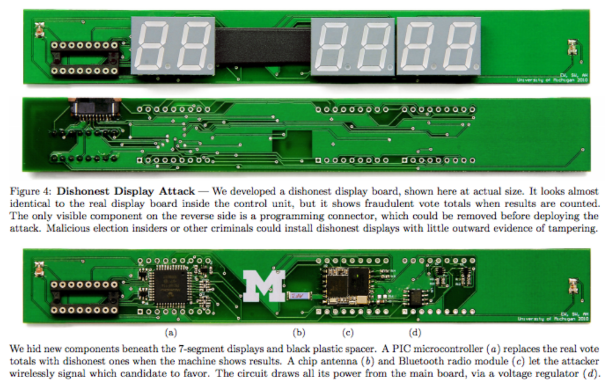
\includegraphics[width=0.8\textwidth]{Imagenes/almacenamiento2}
  \caption{Hardware utilizado}
\end{figure}

Un detalle no menor, es que el recuento de votos de la elección en India se realiza semanas después del sufragio. Por ende, el atacante tiene tiempo para poder realizar el cambio o agregar hardware que le permite realizar el ataque mientras están almacenadas.


\pagebreak
\section{Transmisión de resultados}
La transmisión de votos para su posterior escrutinio también tiene su complejidad ya que la comunicación de estos es sensible a vulnerabilidades y pueden ocurrir ataques.\\
Los casos investigados respecto a los paises Israel e India tienen como particularidad que no transmiten los votos, sino que trasladan las máquinas fisicamente a un lugar y realizan el recuento a mano. \\

\subsection{Voto electronico en CABA (Vot.Ar)}
A continuación haremos referencia al sistema de votación electrónica Vot.Ar utilizado en Argentina en 2015.

\subsubsection{Software o hardware malicioso que puede cambiar la intención del voto, agregar nuevos votos o eliminar votos}
Detalle del ataque multivoto en CABA\footnote{\url{https://docs.google.com/document/d/1aH6kvoLR8O1qWOpEz89FAB2xFcBNB-QqHgZpXxg0vGE/preview}}.

El sistema de almacenamiento de votos en boletas electrónicas en CABA consiste en la grabación del voto en un tag RFID, que luego se utiliza para realizar el conteo de votos de forma electrónica. En este caso la vulnerabilidad proviene de un software mal diseñado y/o implementado que no contiene las debidas consideraciones al momento de leer e interpretar los datos de una boleta.

Más particularmente, puede observarse en una porción del código del sistema de voto electrónico lo siguiente:

\begin{lstlisting}
class Selection(object):
 ...

    def from_string(TAGcontent):
        datatag = parse(TAGcontent)

 ...

      candidates = []
        for e in datatag.vote:
            party_code = e["party"]
            category_code = e["category"]
            candidate = CandidateClass.get(category_code,
                                           party_code)
            candidates.append(candidate)

\end{lstlisting}

Mas allá de una falla de verificacion en la funcion \texttt{parse} mencionada en la bibliografia, lo más grave es que nunca se chequea ninguna de las siguientes cosas:
\begin{itemize}
	\item Unicidad de voto por boleta
	\item Cantidad de votos por candidato sea a lo sumo 1
\end{itemize}

Continuando con la descripción de la vulnerabilidad, en otra sección vital del código, el recuento de votos, se encuentra el siguiente código:

\begin{lstlisting}
class Count(object):

 ...
   def add_selection(self, selection, RFIDserial=None):
        if not RFIDserial or not self.serial_exists(RFIDserial):
            for candidate in selection.candidates:
                self.results[candidate.party_code, candidate.category_code] += 1
            if RFIDserial:
                self._RFIDserials.append(RFIDserial)
  ...
        else:
            raise RepeatedSerial()
\end{lstlisting}

Aquí puede verse una validación sobre la identificación única de cada boleta, pero nunca se realiza la validación pertinente a cada boleta en sí misma acerca de los 2 puntos mencionados anteriormente.

Esta vulnerabilidad, permitía al atacante, escribir sobre una boleta electrónica mediante un smartphone, varios votos a un mismo candidato y esto pasaría desapercibido por ambos módulos del sistema mostrados arriba, constituyendo una fuerte vulnerabilidad.

A continuación se mencionan posibles soluciones a este problema:

\begin{itemize}
	\item Verificar que la escritura de los votos hayan provenido de una máquina real de vot.ar, por ejemplo usando claves privadas
	\item Verificar al momento de la lectura y recuento de la boleta las cuestiones mencionadas
	\item Como método de detección se pueden comparar la cantidad de boletas y la cantidad de votos registrados por máquina
\end{itemize}


\subsubsection{Ataques de denegación de servicio por botnets causando que no se contabilicen votos}

El mecanismo de transmisión de datos utilizado en el sistema Vot.Ar consiste básicamente en una conexión entre cada terminal de votación y un servidor central que recibe los votos.

Si alguien con acceso a la red de alguna máquina de votacion quisiera atacar la disponibilidad del servidor para, por ejemplo, retrasar los resultados, podría obtener la IP o nombre del servidor central y mediante alguna red de botnets obtenida por otro medio, realizar ataques de denegación de servicio y posiblemente explotar vulnerabilidades en el servidor. Por ejemplo podría realizarse un \texttt{SYN-Flood attack}, alterando la disponibilidad del servidor.


\subsubsection{Transmisión de datos y mecanismos de seguridad}
\footnote{\url{http://ivan.barreraoro.com.ar/vot-ar-una-mala-eleccion/}}
\footnote{\url{https://blog.smaldone.com.ar/2016/05/03/el-dia-que-el-sistema-de-voto-electronico-vot-ar-fue-vulnerado/}}
Los mecanismos de transmisión y seguridad propuestos para el sistema Vot.Ar son como siguen:
\begin{itemize}
	\item La terminal de votación es conectada a internet y un técnico de la empresa encargada inicia un software especial de transmisión en ellas. Esta conexión a internet puede variar, desde una conexión cableada del colegio hasta una conexión 3G/4G.
	\item Este software de transmisión se conecta a un servidor de MSA y luego de realizar el recuento físico de boletas apoyando el RFID en la máquina, estos datos se envían al servidor.
\end{itemize}

La propuesta de la empresa para asegurar la transmisión es la utilización de certificados SSL. Cada terminal cuenta con su propio certificado X509 y su clave privada. Esto permite la autenticación de la terminal frente al servidor y es también utilizado para verificar la integridad de los datos.

Claramente es vital que la distribución e instalación de estos certificados en las terminales sea un proceso bien diseñado ya que la información que manejan es muy sensible. Cualquiera que tenga acceso de manera malintencionada a esta información podría hacerse pasar por una terminal y subir datos espurios al servidor.

A continuación se listan algunos de los problemas encontrados en este mecanismo.

\subsubsection{Exceso de confianza en los delegados de instalación de los certificados}

Según las fuentes, los técnicos eran contratados sin ni siquiera una entrevista presencial. Dadas las vulnerabilidades enunciadas a continuación cualquiera de estos técnicos tenía acceso a información que podía comprometer la elección.

\subsubsection{Elecciones defectuosas al momento de distribuir claves privadas}

La distribución de las claves privadas fue encarada de una forma desprolija e insegura.\\

Los certificados estaban accesibles mediante una aplicación web con URLs muy previsibles:\\

\begin{itemize}
	\item \texttt{https://caba.operaciones.com.ar/media/certificados/CABA\_(COMUNA)\_(NUMERO)-(NOMBRE).tar.gz}
\end{itemize}

El acceso a la página era mediante usuario y contraseña de cada técnico, con lo cual, una vez descubierto este patrón, un solo técnico podía descargar todos los certificados.

\subsubsection{Elecciónes defectuosas al momento de asignar contraseñas}
Para empeorar aún mas las cosas, los nombres de usuario y claves de cada técnico eran trivialmente predecibles, ya que consistian en lo siguiente:

\begin{itemize}
	\item Username: (apellido)+(nombre) en minúscula sin caracteres especiales
	\item Password: (emailDelTecnico)
\end{itemize}

Esto estaba especificado en los mismos manuales de capacitación que recibían todos los técnicos. Cualquiera con acceso a alguna planilla de los datos de los técnicos (por ejemplo el personal de RRHH), podrían haber suplantado la identidad de alguno o varios de ellos para cometer ilícitos en su nombre.

\subsubsection{Falta de limitación de poder a un individuo con acceso a los datos}

Estos últimos temas mencionados también deben analizarse en el marco de la confianza que se deposita en una sola persona. Hubiera sido mejor que la responsabilidad hubiera sido compartida entre varias personas, o al menos, las personas responsables deberían ser controladas de algún modo.

\subsubsection{Ataques realizados al sistema de certificados de Vot.Ar}
Dadas las vulnerabilidades mencionadas anteriormente, la lista de certificados fue filtrada días antes del comicio de 2015. Por otro lado se filtraron además los datos personales de los técnicos, haciendo suponer otras vulnerabilidades.

\subsection{Vulnerabilidades en los protocolos de seguridad de las redes}
Lo siguiente fue extraído de un informe de VITA \footnote{(VIRGINIA INFORMATION TECHNOLOGIES AGENCY)} acerca de un sistema de votación utilizado en Virginia, USA \footnote{\url{http://elections.virginia.gov/WebDocs/VotingEquipReport/WINVote-final.pdf}}.\\
Las terminales de votación utilizadas en este sistema, utilizan la red Wifi para comunicarse. Sin embargo, el protocolo de seguridad de la red utilizado es \texttt{WEP}\footnote{Deprecado por la IEEE en 2004}, además, cada terminal \texttt{broadcastea} su nombre de red (SSID) permitiendo un facil escaneo de las terminales. Se realizó un ataque aprovechando este débil esquema de seguridad, que se detalla a continuación.\\
Luego de obtener la lista de nombres de las terminales escaneando las SSID, se procedió a escuchar la red por aproximadamente dos minutos para obtener un \texttt{packet-trace} de la comunicación de red. Utilizando esta información, fue posible explotar una vulnerabilidad del protocolo WEP y crackear la clave, en este caso la clave era \textbf{abcde}. Una vez que se accedió a la red de la terminal, se realizaron análisis de vulnerabilidades con las herramientas NMap\footnote{\url{https://nmap.org/book/man-port-scanning-techniques.html}} y Nessus\footnote{\url{http://www.tenable.com/products/nessus-vulnerability-scanner}}, cuyo resultado mostró que habia varios puertos abiertos y distintas vulnerabilidades. Como se mencionó en la parte de almacenamiento, la combinación de vulnerabilidades en varios frentes de este sistema permitió un reemplazo total de la base de datos de votación de la terminal.

\subsection{Votación por internet: Debilidades en la transmisión de datos}
El envío de boletas para el voto por internet puede pasar por muchos y diferentes servidores, logrando que el sistema no tenga la certeza de que la boleta recibida por el elector, es la boleta emitida para ser usada durante la votación. Además los emails pueden ser interceptados, leídos y modificados en el tránsito violando todos los requerimientos para realizar una votación


% ESTO NO ES SOBRE E-VOTING, ES SOBRE SISTEMAS NORMALES
% Por ejemplo, en Estados Unidos los estándares de transimisión de votos son muy variables. Cada estado elije las máquinas y los métodos para usar y no se rigen por ningún mínimo de seguridad común. Hay un requerimiento estádistico de un error no mayor a 1 en 1 millón, que aparentemente no se cumple\footnote{Douglas W. Jones, \textit{Problems with Voting Systems and the Applicable Standards}, Testimony before the U.S. House of Representatives' Committee on Science, \url{http://homepage.cs.uiowa.edu/~jones/voting/congress.html}}.


\pagebreak
\section{Privacidad del voto}
Como se mencionó en la introducción, la privacidad del voto es fundamental legalmente al proceso electoral. El mayor riesgo es la unificación de un registro de voto con un registro de votante.
El quiebre de la confidencialidad del voto significa que alguien sepa qué es lo que otra persona votó. Es importante evitar que esto sea posible para que cada ciudadano se pueda sentir libre de votar a quién quiera sin presiones. De poder averiguarlo, otras personas podrían tomar represalias o tratar de comprar votos de la población para su conveniencia. Los votos podrían averiguarse en dos instancias: mientras el ciudadno está votando, o a posteriori desde la memoria del aparato o el lugar donde los resultados se almacenaran.
%De igual forma que en Estándares de almacenamiento de votos, mencionaremos distintas técnicas que se utilizaron en distintos países, y los agujeros de seguridad que se encontraron en tales.

\subsection{Identificación del votante a partir de registros}

En todos los sistemas que se analizaron para este trabajo donde se guardan los registros de los votantes, éstos van por separado al voto en sí mismo, para proteger la confidencialidad. Pero si hubiera forma de unir ambas listas, esa seguridad se ve comprometida.

Un ejemplo es Brasil, donde se optó por dejar de utilizar VVPAT debido al incremento del costo por las impresoras y por problemas operacionales. En su lugar, se adoptó un sustituto totalmente digital. Los votos pasaron a almacenarse en una estructura de datos llamada DRV (Digital Record of the Vote) en la memoria electrónica de la maquina de votación. Esta estructura es una tabla separada en secciones, donde cada sección está dedicada a una postulación distinta. Para que no se pueda saber quién voto a quién, esta tabla almacena en distinto orden en que fueron emitidos los votos (La tabla shufflea los votos emitidos)\footnote{\url{https://ivan.barreraoro.com.ar/wp-content/uploads/2015/09/Software-vulnerabilities-in-the-Brazilian-voting-machine.pdf}}.
DRV fue introducido como un reemplazo de VVPAT permitiendo una verificación independiente de los resultados de la elección. Sin embargo, VVPAT es independiente de los votos computados electrónicamente a diferencia de DRV ya que este último es producido por la misma pieza de software que los cuenta. De esta forma, cualquier ataque exitoso al proceso de contar los votos, compromete la integridad de la DRV.

\begin{figure}[h!]
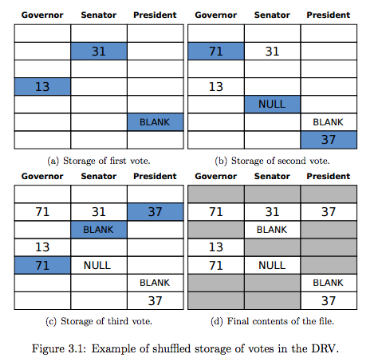
\includegraphics[width=0.5\textwidth]{Imagenes/privacidad1}
\caption{Ejemplo de votos en DRV}
\end{figure}

La ilustración anterior es un ejemplo de una votación utilizando la estructura de datos DRV, donde
\begin{enumerate}
	\item El primer elector vota a la opción 13 como gobernador, a la 31 como senador, y deja el voto en blanco para presidente
	\item El segundo elector vota a la opción 71 como gobernador, impugna su voto para senador, y vota a la opcion 37 como presidente
	\item El tercer y último elector, vota a la opción 71 como gobernador, deja en blanco la de senador y a la opcion 37 como presidente
\end{enumerate}

Se encontraron tres vulnerabilidades:
\begin{enumerate}
	\item Una inadecuada elección del generador de números pseudo-aleatorios. Se utilizan las funciones rand y srand de C que tienen un período muy corto y aceptan solo semillas de 32 bits.
	\item Mala elección de la semilla. La semilla es el horario de apertura de la mesa de votación, que es durante las 7AM y 8AM, dando tan solo 3600 posibilidades.
	\item Semilla pública. No sólo que el proceso de elección de la semilla es determinística, sino que también se la publica en la documentación oficial de la mesa.
\end{enumerate}

Dadas estas vulnerabilidades, se puede realizar los dos siguientes tipos de ataque:
\begin{enumerate}
	\item Ataque directo: Se obtiene la semilla de la documentación oficial de la mesa, y se simula el movimiento de shuffle con N votos y se detecta en qué posición de la DRV fue almacenado cada voto. Esto permite obtener los votos en orden tan solo mirando la documentación oficial. Se pierde el anonimato de la votación si se conoce el orden en que los votantes emitieron sus votos.
	\item Ataque indirecto: Dado los votos fuera de orden, es posible realizar una búsqueda exhaustiva en los posibles valores de semillas, que son 3600, comparando los espacios vacíos.  Con la semilla correcta, se puede realizar el primer ataque
\end{enumerate}

En las EVM en India\footnote{\url{https://jhalderm.com/pub/papers/evm-ccs10.pdf}}, existe un ataque que afecta a la privacidad del voto llamado Clip-on Memory Manipulator Attack. A diferencia del ataque mencionado en una sección anterior en el que se intercambia una placa, en este se agrega temporalmente nuevo hardware a la máquina que registra los votos, permitiendo dos ataques: robar votos y violar el secreto del voto.
\begin{figure}[h!]
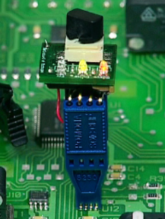
\includegraphics{Imagenes/privacidad2}
\caption{Hardware a agregar. Al girar la perilla, se indica que candidato favorecer}
\end{figure}


\subsection{Acceso ilegítimo al momento de votar}

Este tipo de ataques consisten en averiguar el voto mientras la persona está sufragando. Este tipo de quiebre de confidencialidad es especialmente problemático porque contradice uno de los principales beneficios del voto electrónico que es que la gente con discapacidades visuales o motrices pueda efectuar su voto sin ayuda de otra persona, y por lo tanto, en secreto.

Una de las formas de violar este principio es a través de la lectura de formas de almacenamiento externo, como la BUE en la ciudad de Buenos Aires donde existen dos posibles ataques que comprometen la privacidad del voto\footnote{\url{http://ivan.barreraoro.com.ar/vot-ar-una-mala-eleccion/}}.

El primero es que se pierde el anonimato del voto, ya que el voto se escribe en el chip RFID de una BUE y se puede leer el contenido de estos chip a cierta distancia sin que el votante se entere. No solo eso, sino que también cada chip RFID tiene un número que lo identifica. Por ende, si sabemos el orden en que los electores votan y se les da una BUE con un orden predeterminado podemos, al finalizar, revisar el número del RFID, saber a qué elector pertenece y su voto\footnote{\url{https://blog.smaldone.com.ar/2016/01/08/sobre-el-chip-rfid-de-la-boleta-unica-electronica/}}.

El segundo posible ataque también corresponde a la pérdida del anonimato del voto pero no se utiliza esta vez el chip RFID, sino la memoria EEPROM integrada de 256KB que se encuentran en el microcontrolador ARM. En esta memoria se puede almacenar todo tipo de información, como por ejemplo el voto y una marca de tiempo. Por ende, similar al anterior, con conocer el orden de los electores al votar se puede saber las elecciones de los electores.

Otro ejemplo de lectura posible de los votos en la urna es en el sistema israelí (que es muy parecido al usado en Argentina)\footnote{\url{https://iss.oy.ne.ro/e-Voting-Jamming.pdf}}\footnote{\url{http://www.eng.tau.ac.il/~yash/evoting-relay-rfid2010.pdf}}. Éste se denomina ``relay attack'', donde la comunicación con las dos partes es iniciada por el atacante que luego simplemente transmite mensajes entre las dos partes sin manipularlas ni siquiera necesariamente leerlos, hasta obtener su objetivo.

Un ejemplo de un relay attack
\footnote{\url{https://en.wikipedia.org/wiki/Relay_attack}}
 es que Peggy trabaja en un edificio de alta seguridad que se accede utilizando una tarjeta inteligente en su bolso. Cuando se acerca a la puerta del edificio, el edificio detecta la presencia de una tarjeta inteligente e inicia un intercambio de mensajes para verificar que la tarjeta es de Peggy. El edificio le permite a Peggy entrar. Mallory quiere entrar en el edificio. Mallory se acerca al edificio con un dispositivo que simula una tarjeta inteligente, y el edificio responde iniciando el intercambio de mensajes. Mallory reenvía el mensaje a su cómplice Evelyn que está siguiendo a Peggy mientras hace mandados en otra parte de la ciudad. Evelyn retransmite el mensaje a la tarjeta inteligente de Peggy, escucha la respuesta de la tarjeta inteligente de Peggy, y envía la respuesta a Mallory, que la transmite al edificio. Continuando de esta manera, Mallory y Evelyn transmiten los mensajes entre el edificio y la tarjeta inteligente de Peggy hasta que el edificio esté satisfecho de que se está comunicando con tarjeta inteligente de Peggy. El edificio se abre y entra Mallory.

Esta implementación israelí sufre los siguientes ataques:
\begin{itemize}
	\item Ballot sniffing attack, el cual permite leer todos los votos en la urna en cualquier momento. Al realizar este ataque antes de que un elector vote, y acto seguido de que el elector votó sin que nadie más haya votado aún, se puede saber a quién votó el elector afectando el anonimato del voto.
Para realizar este ataque, un retransmisor se establece entre los votos dentro de la urna y la terminal de verificación dentro de la cabina de votación que se encarga de retransmitir el contenido de los votos de la urna a la terminal de verificación para saber su contenido. Se activa repetidamente la terminal de verificación, cada vez con una votó diferente y se almacena su respuesta
\begin{figure}[h!]
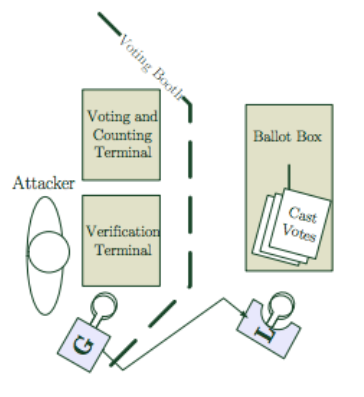
\includegraphics{Imagenes/privacidad3}
\caption{Ballot sniffing attack}
\end{figure}
	\item Single dissident attack, el cual permite suprimir votos.

	\item Zapping attack, el cual permite anular los votos de una urna

	\item Jamming attack, el cual permite interrumpir la operacion de una terminal de voto electronico a distancia

	\item Fault attack, el cual hace que la estación se encuentre en un estado inválido y luego dándola de baja

\end{itemize}

Para los dos primeros ataques, es necesario un retransmisor.

Israel, un país conocido por su desarrollo rápido y continuo de la tecnología, tuvo la oportunidad de poner en práctica el voto electrónico ya en 2008

\footnote{\url{http://e-lected.blogspot.com.ar/2013/03/the-implementation-of-e-voting-in.html?m=1}}.

. Sin embargo, a pesar de la aprobación en general de la clase política, esto no sucedió, y en la actualidad el país no lo usa. ¿Por qué? Israel es un ejemplo de los riesgos que corre un país cuando su proceso de modernización electoral no es transparente y abierto a la gente.

En 2008, el Ministerio del Interior israelí publicó una propuesta de ley para la implementación del voto electrónico en los próximos eventos electorales después de una prueba exitosa en paralelo a las elecciones locales de 2007. Sin embargo, esta propuesta plantea dos problemas: en primer lugar, no hubo una discusión pública sobre el asunto, y todo se hizo a puerta cerrada; segundo, las máquinas de votación del país que querían usar no emiten recibos de voto, lo que hizo que el electorado sospechoso de su auditabilidad.

Se demostró que contenía vulnerabilidades, y la falta de medios para auditabilidad .
Al final, tras las protestas de los ciudadanos en tensión, la iniciativa de votación electrónica fue cancelada e Israel tuvo que volver a votación manual.


Por último, y bastante más complicado, está el ejemplo de la auditoría holandesa(http://wijvertrouwenstemcomputersniet.nl/images/9/91/Es3b-en.pdf), donde se logró identificar el voto mientras sucedía a través de un ``side-effect'' muy interesante: la frecuencia de radio. En este ataque, se logró encontrar una señal a varias frecuencias distintas, representada como un zumbido, y se dilucidó que la frecuencia cambiaba si el texto a mostrar por pantalla tenía caracteres especiales porque el controlador utilizado para mostrarlos necesitaba hacer más trabajo. En particular, en los Países Bajos al momento de la auditoría uno de los partidos más importantes tenía un caracter acentuado y el otro no, con lo que se podía saber de oído (con cierto aparato para escuchar la frecuencia) por las emisiones de la máquina si un votante elije a cierto partido.

Con un poco más de trabajo, analizando las emisiones irradiadas por la pantalla en más detalle, se pudieron identificar todos los candidatos por separado, pero en la auditoría se aclaraba que ese nivel de trabajo no era factible a ser realizado al momento de la elección estando suficientemente cerca de la máquina.



\pagebreak
\section{Auditabilidad del sistema}
Cuando se habla de auditabilidad se habla de las posibilidades de realizar análisis sobre cómo funciona un sistema y cómo se llegó a un cierto resultado. Hablando de sistemas de votación esto puede querer decir la capacidad de analizar el software y el hardware que realiza la elección para saber cómo funciona, si es seguro o qué problemas puede tener; o puede referirse a auditar los resultados de una elección, saber cómo se llegó a un cierto resultado y tener alguna verificación de que ese resultado es coherente con la realidad.

\subsection{Auditoría del resultado con comprobantes en papel}

Este tipo de auditorías son encargadas por las autoridades, ya sea el tribunal encargado de las elecciones, o un juez si hubiera un resultado disputado, y consisten en contabilizar los comprobantes de los votos en papel para compararlos con los registrados electrónicamente\cite{postElection}. El resultado válido finalmente, si ambos no coincidieran, es el resultante del voto manual. Del tipo de tecnología que requiere esta clase de auditorías se va a hablar mejor en la próxima sección.

\subsection{Auditorías de seguridad realizadas por profesionales}

Esta clase de auditorías puede ser encargada por las autoridades encargadas de la elección o puede ser realizada de forma independiente por expertos que hayan conseguido acceso a una máquina de votación o al software pertinente. El objetivo principal de estas auditorías suele ser encontrar agujeros de seguridad que permitan la modificación de los resultados de la elección por un usuario malicioso. Por supuesto, quién realiza la auditoría puede tener intereses políticos que lo induzcan a presentar un resultado más o menos favorable a las autoridades del momento, pero en este trabajo vamos a evaluar el foco técnico de los análisis.

\subsubsection{Verificación de cambios en el software instalado}

Uno de los focos de la auditoría es que el software no pueda ser, o no haya sido, modificado durante la elección. Son casos separados a nivel investigativo. Es posible verificar que el software sea el mismo antes y después de la votación haciendo comparaciones justo antes y justo después de la elección. De esta forma podría ser detectable algún tipo de interferencia en el software. Código o ejecutables modificados, archivos agregados a la máquina que no estaban allí, o que no se previera que estuvieran allí. Las comparaciones entre la memoria pre elección y post elección se pueden hacer comparando imágenes (dumps) bit a bit (por ejemplo con un software llamado GEMS) o comparando archivos, timestamps y buscando contenido malicioso conocido o comportamiento sospechoso.

Hay ciertas máquinas usadas en parte de Estados Unidos que son de lectura automática de boletas en papel. Estas máquinas son comunes a varios estados, pero para ajustarlas a las particularidades legales de cada uno, aceptan una memoria externa con un programa exclusivo de cada estado. La Universidad de Connecticut ha realizado, y sugiere la realización, de este tipo de auditorías para las memorias externas. Se supone que éstas son el equivalente a una urna en forma electrónica \cite{preElection}, ya que contienen el código exclusivo, los datos de los candidatos y partidos, el esquema de votación y la contabilización de los votos.
En estas auditorías, el equipo hizo comparaciones de imagen bit a bit con el firmware de las máquinas de lectura de las boletas, y luego análisis más detallado sobre las memorias, pre y post elección. Para ver que no hubiera datos modificados que no debieran estarlo (como los datos de los candidatos), que los contadores estuvieran en 0 antes y en números razonables después, y que el estado final fuese consistente.

\subsubsection{Revisiones pre elección}

Un sistema de elección que ya está en uso, igual debe ser auditado previo a cada elección. Así como en la sección anterior se discutía el hacer un análisis bit a bit del software comparando si es el mismo entre el principio y el final de la elección para prevenir que alguien haya intervenido durante el día, también se debe tener en cuenta la posibilidad de que alguien lo hubiera intervenido previo a abrir la elección. Se debe conocer cuál es el software que debe tener una máquina, y se debe verificar antes de abrir la elección que efectivamente sea ese\cite{holanda}.
El momento de la verificación es sensible, ya que a partir de ahí cualquier persona con acceso a las máquinas podría interferirlas sin ser visto, pero esto está más relacionado con la custodia de las máquinas y fue discutido con anterioridad. Si la máquina tiene algún puerto abierto, se hace más difícil controlar que no pueda ser accedida, pero se puede intentar asegurar los componentes físicos con sellos tamper-proof, y entrenando a los custodios y autoridades de mesa para descubrir alteraciones al hardware.

\subsubsection{Auditorías de evaluación del sistema}

Previo a usar cualquier sistema por primera vez para una elección, se debería auditar por un profesional que juzgue si el sistema cumple con su objetivo, es seguro y a prueba de intentos maliciosos de ataque. “Debería” no porque haya necesariamente algún parámetro legal, si no porque el acto eleccionario se basa en la confianza de los votantes para con el sistema. Es fundamental para la legitimidad del gobernante que asuma como ganador de esas elecciones que los votantes confíen en la transparencia de la elección.

Este tipo de auditoría puede ser realizada por iniciativa de las autoridades a cargo de la elección\cite{righetti}, por iniciative de un organismo independiente que solicite la información necesaria y acceso a las máquinas\cite{holanda}\cite{itba} o por iniciativa de algún particular que tenga acceso como pueda al sistema en cuestión\cite{votar}.
Los principales destinatarios del informe resultante de una auditoría son el organismo gubernamental encargado de la reglamentación e implementación de las elecciones, y el fabricante de las máquinas utilizadas y/o su software. Este informe contendrá al menos una explicación de todos los análisis realizados sobre el sistema, los resultados de cada uno, y una profundización sobre aquellos puntos donde se hayan encontrado problemas. Probablemente finalizando con una lista de sugerencias sobre cómo atacar los problemas encontrados y algún tipo de valoración sobre si la máquina es suficientemente segura como para ser utilizada en elecciones o no.

Para que una auditoría pueda ser completa, los organismos a cargo deben proveer todo el material involucrado y hacerse presentes para contestar las dudas que pudieran ocurrir. Estos materiales probablemente incluyan: hardware, software ejecutable (en su última versión), código fuente de ese software, documentación, boletas de papel, impresoras, identificación (llaves, tarjetas, pines). De faltar algún componente importante del sistema, la validez de la auditoría podría verse comprometida (ITBA).

Al momento de las elecciones será decisión de las autoridades escuchar las auditorías o no. En el caso argentino, las auditorías progresivas realizadas por la FCEN fueron tenidas en cuenta para realizar modificaciones en el software de las máquinas, pero no así la auditoría independiente que recomendaba no usar el voto electrónico. En Países Bajos, máquinas de la empresa Nedap fueron utilizadas durante algunos años hasta que un grupo autodenominado “We do not trust voting computers” (“No confiamos en las máquinas de votación”) logró romper la seguridad de la máquina de forma muy sencilla y salió a hacer campaña en los medios de comunicación. Eventualmente, en 2007, se prohibió el voto electrónico en todo el país\cite{holanda}.


\pagebreak
\section{Comprobantes}
En inglés se habla de un “paper trail”, literalmente “rastro de papel”, cuando una operación realizada tiene comprobantes en papel verifican que se realizó y cuál fue el resultado. En el acto de votación electrónica este rastro de papel es siempre un adicional a los registros guardados por las varias máquinas encargadas de realizar la elección y tiene la ventaja de ser entendible para cualquiera (sin necesidad de entrenamiento en informática), posiblemente duradero en el tiempo, y de funcionar como back up en caso de que algo fallara con el sistema electrónico.

Hay dos momentos del proceso de votación donde el votante necesita algún tipo de comprobación de su acto: por un lado, al emitir el voto es necesario saber que el proceso fue exitoso y finalizó; y por el otro (y esto no sucede cuando se vota con boletas de papel) el votante puede querer comprobar que efectivamente su voto se contó, y se contó para el candidato elegido. Los sistemas de votación ‘End-to-end’ le permiten verificar ambas instancias.

\subsection{Ejemplo de un End-to-end diseñado recientemente}

Desarrollado en Texas para suplir las fallas de las máquinas DRE compradas 10 años antes, y frente a reticencia de las autoridades a volver a boletas con marcas manuales que ya les habían traído problemas de ambigüedad en el pasado.
El sistema consiste en software diseñado para ser usado sobre hardware comercial, y para permitir que el votante pueda verificar su voto (además de algunos “constraints” más dados por la forma de las elecciones en Estados Unidos, como múltiples días de votación y grandes cantidades listas de candidatos)\cite{star}.

El diseño de este sistema incluye back ups en papel en todas las instancias: al llegar, el votante se registra con su documento y recibe un sticker duplicado con un código de barras. Una de las copias queda en un registro en papel con su firma, y la segunda se escanea en la máquina controladora de la red interna del centro de votación. Esa computadora le entrega un PIN de 5 dígitos, único a esa central, que el usuario ingresará en la máquina de votación propiamente dicha. Al terminar de votar recibirá un “ticket” con dos copias de su voto, una en texto plano con un número de secuencia identificatorio, y otra con un hash del voto encriptado y la fecha, hora e identificador del lugar de votación. El votante deposita la que tiene el voto en claro (luego de verificar que sea el correcto) en la urna, y se queda con el otro. Si el voto no es depositado allí, no es válido. Con el hash que se llevó en la segunda copia, el votante puede entrar en el sitio del condado y verificar que se haya contado como válido.

El hash que se lleva el votante es de la siguiente forma: $z_i = H(E_K(v),m,z_i-1)$ con $H$ la función de hash, $E_k$ el algoritmo de encriptación, $m$ el identificador de la terminal de votación y $z_i - 1$ el hash anterior. De esta forma el hash no contiene la información del voto en forma directa.

Estos hashes se conservan en la máquina con un timestamp del momento en que se realizó el voto, y las claves de encriptación se guardan fuera del sistema, combinando claves públicas de un número determinado de oficiales administrativos de la votación.

Este sistema de votación tiene un rastro muy completo del proceso, pero notablemente, no funciona sólo como back up si no que agrega una medida de seguridad extra: no se cuenta ningún voto registrado electrónicamente si el número de serie equivalente no está en la urna física. Esto anula la posibilidad de modificar los votos guardados en la máquina de forma que se multipliquen o pensar en un ataque que borre los votos guardados ya que la urna se abre de todos modos y es la que tiene el dicho final sobre qué votos se cuentan.

De haber alguna discrepancia de votos, es relativamente fácil aislarla a algún voto en particular.

\subsection{Sistemas electrónicos sobre boleta de papel}
Otro tipo de sistema end-to-end en Estados Unidos, es Scantegrity\cite{scantegrity} o Prêt à Voter, que agregan una capa de inteligencia electrónica a un sistema de boletas anotadas a mano.
El objetivo de Scantegrity era reemplazar los DRE en uso y mejorar las boletas en papel leídas y contadas en forma electrónica con el agregado de un rastro de papel.
El sistema ofrece seguridad para el votante de que su elección fue contada proveyendo un comprobante de voto con un número de serie y un código identificatorio de su candidato. Los códigos son asignados en cada boleta impresa al azar y sólo son visibles cuando el votante marca en la boleta con un marcador especial que revela la “tinta invisible”. El votante luego copia ese código a una porción removible de la boleta. Una vez que el voto fue aceptado por las autoridades de mesa, éstos pasan un marcador con otra tinta especial por el sector removible para que quede visible el número de serie de la boleta, y el votante se lleva este comprobante. Al finalizar la elección éste puede chequear en el sitio del condado que el número de serie de su boleta esté asociado al código que anotó como el correspondiente a su candidato. Los resultados de la elección se calculan de forma reproducible a partir de los publicados en internet, pero la lectura de las boletas se sigue haciendo en forma automatizada con los lectores ya existentes.

Los riesgos posibles con respecto a la generación de comprobantes son dos: que el comprobante contenga información respecto del voto, rompiendo la confidencialidad del acto y posibilitando la venta de votos; y la alteración del resultado final de la elección convenciendo al votante de que votó por quién quería cuando en realidad se generó otro voto.
En este paper\cite{kelsey} se describe una forma de reemplazar las boletas de Pret a Voter por unas falsas para que el código ingresado no sea el deseado, si no el de un candidato en particular. Este ataque no es técnicamente informático, si no que depende de los administrativos que entregan las boletas y la forma de “ticket” que elija el votante.


\subsection{Problemas de usabilidad}

Idealmente, es deseable implementar todo aquello que vuelva al sistema más seguro. Pero en la práctica hay otros factores que afectan sobre la decisión de agregar características nuevas al sistema de votación. En particular, hay un estudio hecho sobre los sistemas mencionados que funcionan como agregado a las boletas de papel que, si bien ayudan estrictamente hablando de seguridad, son tan difíciles de usar para los votantes que el porcentaje de votos exitosos puede ser tan bajo como el 58\%\cite{usability}. Esto quiere decir que un porcentaje importante de los votantes no puede elegir a un candidato exitosamente porque no comprendió el uso correcto de alguna porción del sistema. Así mismo, registraron tiempos más largos de uso y niveles de frustración altos entre las personas testeadas. Y agregan que la cantidad de gente que efectivamente realiza la verificación posterior de su voto es muy baja.

\subsection{Paper trails parciales}

Fuera del contexto de los sistemas end-to-end hay otras opciones utilizadas. Hay sistemas que utilizan papel en forma parcial, por ejemplo, combinando una impresora con un DRE, que devuelve un comprobante del voto que le permite al votante verificar que fuera el candidato correcto. En ocasiones, ese comprobante puede ser metido en una urna y usado para contabilizar votos de haber problema con el sistema electrónico, pero no es siempre así.

En el caso de que la impresión sea utilizada como backup al sistema electrónico guardándose para posterior verificación, el sistema se denomina VVPAT (Voter-verified paper audit trail), este es el tipo de sistema a implementarse en india\cite{indianExpress} y en uso en algunos estados de Estados Unidos\cite{nevada}. Este tipo de sistemas no le permiten saber al votante si su voto se contó, pero dan un respaldo en caso de haber habido problemas con el resultado electrónico, incluyendo si fuera necesario hacer el recuento de nuevo.
Se implementa de varias formas distintas: puede ser que el votante tenga que cortar el recibo y depositarlo en una urna, como en STAR, o puede ser que el votante nunca toque el recibo, pero si lo vea a través de un cristal para verificarlo, como se hace en Nevada, EEUU\cite{saltman}.

El caso de la Ciudad de Buenos Aires es un VVPAT con ciertas limitaciones. Por un lado, sirve para verificar que el candidato seleccionado es el mismo que figura en la boleta, gracias a la impresión del voto en texto plano, pero no se utiliza el valor impreso en la boleta, si no el que está en el chip que lee la misma máquina para contar\cite{votar}. De forma que las boletas en papel no están sirviendo como verificación a menos que haya un recuento específico.


\subsection{Lugares sin paper trail}

Las máquinas utilizadas en algunas partes de Estados Unidos\cite{stanfordNews} y en todo Brasil son DRE, que como se viene viendo, no entrega ningún tipo de comprobante por sí sola\cite{aranha}. El hecho de que no imprimen ni usan papel se comunica como ventaja a nivel de ahorro de recursos.

En Nevada se vio como una deficiencia de seguridad no tener ningún backup al conteo electrónico, fue ese el estado del que se habló más arriba, y por eso implementó una combinación de DREs con impresoras para generar un VVPAT. Varios otros estados siguieron su ejemplo, como California uno de los estados con más representantes del país, y se está extendiendo por el territorio.

\subsection{Objeciones al paper trail como se implementa habitualmente}

Si bien la literatura parece estar en acuerdo sobre la necesidad de mantener un rastro de papel de las elecciones, hay discusiones existentes sobre la forma de implementarlo. Por un lado, hay algunos autores que remarcan que las máquinas tienen grandes beneficios de accesibilidad, pero que éstos son contrarrestados agregando un recibo de papel con un formato distinto al de la pantalla, en ocasiones muy largo. Todo esto podría dificultar la verificación por personas con limitaciones de lecto-escritura, quienes tuvieran problemas de movilidad o de visión\cite{saltman}.


\pagebreak
\section{Apéndice: Los requerimientos mínimos para sistemas de voto electrónico en la votación llevada a cabo en C.A.B.A. Julio 2015 (Johns Hopkins University)}
\textit{Movilidad y accesibilidad:} “Un votante no debería estar restringido a votar en un solo lugar”. Lo relacionamos con garantizar la disponibilidad. En la realidad y a nivel nacional, se lo designa a un solo lugar, pero las máquinas no hacen un chequeo de esto. Por lo tanto, se estaría permitiendo este fundamento. Según el Gobierno de la Ciudad de Buenos Aires, el padrón electoral no se ha digitalizado. (FAQ 11, GCBA Boleta electrónica). Tampoco se limitan los votantes una máquina únicamente, ante un caso de falla o inutilización de la misma, debería ser fácilmente reemplazables. El gobierno de la ciudad afirma que esto es posible (FAQ 3, GCBA Boleta electrónica).
En cuanto a los votantes con discapacidades, el sistema debe facilitar y hacer posible el uso para los mismos. Según el GCBA, se puede activar un modo de alto contraste, o sino un teclado físico especial en braille con audífonos para mantener la privacidad del votante y escuchar instrucciones. En cuanto a seguridad, comprendemos que debe tener en cuenta dos cosas. Garantizar el acceso a todos los votantes y además, no generar vulnerabilidades habilitando estos modos. Utilizando una máquina que garantice todo lo expresado anteriormente, ayuda a garantizar el voto universal y secreto.

\textit{Conveniente:} el sistema debería permitir al votante emitir el voto de forma rápida, en una sesión, y no requerir habilidades especiales, ni intimidar al votante. (Ley 4894 C.A.B.A., artículo 24, inciso a). Previo utilización del sistema electrónico, se pusieron puntos de capacitación o consulta sobre la utilización del mismo. Lo que podría ser cuestionable es el tiempo previo al mismo para garantizar este fundamento. La Defensoría del Pueblo, lanzó unos pocos meses antes una campaña de capacitación, abril del 2015 (http://www.defensoria.org.ar/biblioteca/, informe anual 2015). Así mismo, se hicieron accesibles las supuestas máquinas a utilizar, lo que facilita un primer vistazo a posibles vulnerabilidades de las mismas por parte de algún posible atacante. Como por ejemplo, si tienen expuestos puertos o entrada y salida de medios. Por otra parte, las indicaciones visibles, de cómo utilizar la máquina tienen que ser fáciles de interpretar. (Ley 4894 C.A.B.A., artículo 24, inciso f)

\textit{Unicidad:} un votante puede votar una única vez. El control del mismo se realiza al igual que la elegibilidad. El identificador de una boleta no está asociado al votante una vez insertado la boleta impresa en la urna. El control lo hacen las autoridades de mesa, que deben brindar una única boleta al votante.

\textit{Autenticidad del votante, elegibilidad:} se tiene que asegurar que el votante se identifique. Se realiza de forma personal. Una vez identificado, se le entrega una única boleta. Si no se identifica, no debería votar. Nuevamente, el control es humano.

\textit{El voto secreto del votante:} como la ley establece que el voto es secreto, el sistema debe de garantizar esto. El sistema utilizado en C.A.B.A. asegura que garantiza el mismo ya que las máquinas no poseen memoria que grabe información del voto y la boleta al doblarse correctamente, posee una protección contra lecturas externas. Solo abriéndose y apoyándola en una máquina lectora, se puede conocer el voto. A su vez, una vez introducida la boleta en la urna, se pierde la relación de la boleta con el votante. (FAQ GCBA Boleta electrónica). La boleta no almacena ninguna información propia del votante.
En un informe del Poder Ciudadano, sobre las elecciones en Salta (mismo sistema usado en las elecciones de la Ciudad de Buenos Aires), se destacó como una gran debilidad la pérdida del voto secreto. Se reportó que, personas con discapacidad, requirieron de ayuda para poder emitir su voto. La asistencia fue sin una distancia prudente. La accesibilidad del sufragio debe garantizarse con el ejercicio individual del voto.

\textit{Integridad:} este fundamento también aparece en la ley (Ley 4894 C.A.B.A., artículo 24, inciso g) del voto en CABA. Las máquinas no tienen almacenamiento ni guardan información de la votación, por lo que la integridad de las mismas se corresponde a la integridad del software que ejecutan. El mismo viene en un DVD, sellado con un hash disponible para verificar la integridad del mismo. El hash del contenido era con md5 luego cambiado a SHA512, pero no se utiliza. El contenido hasheado se almacenaba en un archivo que puede ser generado por cualquier persona. No está firmado digitalmente, dando cuenta de un grave error de apreciación de seguridad. (informe Smaldone). Así mismo, el hash del DVD se almacena en el propio DVD, otro gravísimo error, ya que alcanza con que alguien modificara el DVD, calculara el nuevo hash y lo pusiera en el mismo lugar. Las autoridades de mesa no podrían verificar la integridad del mismo con respecto del DVD oficial.
En el caso de la boleta electrónica, posee una memoria que permite la posibilidad de una única escritura, bloqueando otras posibles cuando se intentara grabar. La responsabilidad es de quien graba la información por primera vez. Por lo que, si bien las máquinas utilizadas activaban dicho bloqueo, si un usuario pudiese violar la máquina, podría hacer que no se active la escritura única, pudiendo modificar información ya almacenada en la BUE (boleta única electrónica), según el informe de Smaldone donde se hace referencia al manual del chip RFID utilizado. La importancia de la escritura única es garantizar la integridad de un voto ya emitido, bloqueando cualquier intento de cambiar el contenido del voto.
Como se mostró, el equipo utilizado permite un fácil acceso a los puertos USB, lectora de DVD, etc. Lo que uno podría insertar un software para modificar el normal funcionamiento del sistema y corromper el la información que se muestra con la que se imprime en la boleta.
En la auditoría de la FCEN, se destaca que todos los procesos que se ejecutan en la máquina, corren con nivel de root. Por lo que, si un usuario con acceso a la máquina logra aprovechar alguna vulnerabilidad, puede obtener control total del sistema y modificar su comportamiento oficial. Por ejemplo, imprimir cierto valor en la boleta y mostrar otro por pantalla. Al tener ciertos puertos y medios fácilmente accesibles, esto es posible, por ejemplo, explotando vulnerabilidades de los puertos USB.

\textit{Privacidad:} Nadie debería poder determinar el voto de un votante. No existe una relación estricta entre la boleta y el votante, la boleta la elige el votante al azar. Una vez insertada en la urna, se pierda la relación votante/boleta. Además, la máquina no almacena votos por lo que la privacidad, se podría ver amenazada únicamente si lee la boleta a distancia cuando la posee el votante.Según las especificaciones del fabricante de los chips RFID, es posible. (https://blog.smaldone.com.ar/2016/01/08/sobre-el-chip-rfid-de-la-boleta-unica-electronica/). Aunque el GCBA, afirma que se utiliza un film metálico para evitar la lectura de la BUE si está bien doblada.

\textit{Testeo y Certificación:} las máquinas utilizadas no son certificadas. Gran diferencia con Estados Unidos, donde la National Institute of Standards and Technology determina que cada Estado fije distintos grados mínimos de testeo y certificaciones. A su vez, desarrollaron una guía para implementar distintas políticas de seguridad. A nivel local, no hubo una política fuerte por parte del Estado o de la Justicia para garantizar que se cumplan con las políticas de seguridad definidas en la Ley. Hubo resistencia por parte de la empresa MSA para brindar información y prestarse para la auditoría previa, durante y posterior a la elección (Informes en distintos medios y Smaldone).


\pagebreak
\section{Conclusiones}

\pagebreak
\printbibliography


\end{document}
